\section{Números Complejos}

    \subsection{Operación Fundamentales}


        Para realizar operaciones en números complejos, se establece una independencia lineal entre los números reales e imaginarios, esto permite realizar las operaciones básicas de la siguiente forma

        \begin{enumerate}
            \item \textit{Suma}
                \begin{equation*}
                    z_1 + z_2 = (a + ib) + (c + id) = (a + c) + i (b + d)
                \end{equation*}
            \item \textit{Resta}
                \begin{equation*}
                    z_1 - z_2 = (a + ib) - (c + id) = (a - c) + i (b - d)
                \end{equation*}
            \item \textit{Multiplicación}
                \begin{equation*}
                    z_1z_2 = (a + ib)(c + id) = (ac - bd) + i(ad + bc)
                \end{equation*}
            \item \textit{División}
                \begin{equation*}
                    z_1/z_2 = (a + ib)/(c + id) = \frac{(ac + bd) + i((bc-ad))}{c^2+d^2}  
                \end{equation*}        
        \end{enumerate}

        Vale la pena recalcar que números complejos cumplen con las propiedades  \textbf{Conmutativa} y \textbf{asociativa}, tanto para la suma como para la multiplicación, adicionalmente también se cumple que el $0$ es modulo para la suma y $1$ para la multiplicación. Por último, se tiene que para todo $z_1 \neq 0$ existe un único $z$ tal que $z_1z = zz_1 = 1$, donde $z$ es llamado el inverso multiplicativo de $z_1$.
    
    \subsection{Números complejos en Forma Polar.}

        Como se expresó anteriormente, los números complejos pueden ser expresados como bases vectorial de un espacio $\mathbb{R}^2$, esto permite establecer una descripción de los complejos en términos de $r$ y $\theta$.

        \begin{wrapfigure}{l}{0.4\textwidth}
            \centering
            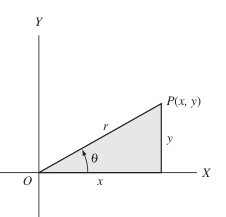
\includegraphics[width=0.4\textwidth]{imgs/ipolar.png}
            \caption{}
            \label{fig:ipl}
        \end{wrapfigure}
        Esta representación se realiza en el \textit{plano complejo} o \textit{diagrama de Argand}, donde a cada número complejo le corresponde un único punto en el plano complejo. Los ejes de este espacio son llamados eje real (para el $X$) e imaginario (para el eje $Y$).
        \vspace{0.5cm}

        Deacuerdo con Fig.\ref*{fig:ipl} para un punto $P$ se pueden establecer las siguientes relaciones

        \begin{align*}
            x = r\cos\theta &  & y = r\sin\theta
        \end{align*}

        donde $r = \sqrt{x^2 + y^2}$ es definido como el modulo de $z$, el cual se denota como $|z|$. Esto hace posible escribir entonces el número complejo en terminos de $r$ y $\theta$.

        \begin{equation*}
            z = x + iy = \cos\theta + i\sin\theta
        \end{equation*}

        Adicionalmente el ángulo $\theta$ es conocido como la fase del número complejo y tiene la forma de $\theta = \arctan(y/x)$. Usando la analogia vectorial es posible demostrar la relación existente entre los modulos de un número complejo (Ver Problema 1 - Tarea 01). Por otro lado, los modulos y fases de números complejos cumplen,
        
        \begin{gather*}
            |z_1 z_2 | = |z_1||z_2|\\
            \arg(z_1z_2) = \arg z_1 + \arg z_2
        \end{gather*}

        Donde $\arg$ es ángulo que forma el número complejo con el eje real. Otra forma bastante útil de calcular el modulo de un número complejo es mediante el complejo conjugado el cual esta definido como el cambio de signo de la parte imaginaria, es decir 

        \begin{equation*}
            z^{*} = x - iy 
        \end{equation*}

        Por tanto el modulo será 

        \begin{equation*}
            |z| = \sqrt{zz^{*}}
        \end{equation*}

    \subsection{Teorema de DeMoivre}

        Si se definen dos números complejos $z_1 = r_1(\cos\theta_1 + i\sin\theta_1)$ y $z_2 = r_2(\cos\theta_2 + i\sin\theta_2)$ tal que 

        \begin{gather*}
            z_1z_2 = r_1r_2(\cos(\theta_1 + \theta_2)+ i\sin{\theta_1 + \theta_2})\\
            z_1/z_2 = r_1r_2(\cos(\theta_1 - \theta_2)+ i\sin{\theta_1 - \theta_2})\\
        \end{gather*}

        y mediante indución matemática se generaliza este resultado se obtiene,

        \begin{gather*}
            z_1z_2\dots z_n = r_1r_2\dots r_n\left[\cos(\theta_1 + \theta_2 + \dots + \theta_n) + i\sin(\theta_1 + \theta_2 + \dots + \theta_n)\right]\\
            z^{n} = r^{n}\left(\cos\theta + i\sin\theta\right)^{n} = r^{n}(\cos{n\theta}+ i\sin{n\theta})
        \end{gather*}

        Esta última ecuación es conocida como \textit{Teorema de DeMoivre}, el cual es útil para calcular raices de números complejos. Si se quiere calcular la n-ésima raíz de un complejo

        \begin{gather*}
            z^{n} = r^{1/n}\left(\cos\theta + i\sin\theta\right)^{1/n} = r^{1/n}(\cos{(\theta/n)}+ i\sin{(\theta/n)})\\
        \end{gather*}

        Ahora como para una n-raíz deben existir $n$ valores diferentes para $z^{1/n}$

        \begin{equation*}
            z^{n} = r^{1/n}\left(\cos\theta + i\sin\theta\right)^{1/n} = r^{1/n}\left[\cos\left(\frac{\theta + 2k\pi}{n}\right) + i \sin\left(\frac{\theta + 2k\pi}{n}\right)\right]
        \end{equation*}

        Con $k = 0,1,2, \dots, n-1$ 

    \subsection{Ecuación de Euler}

        Considerando la expasión en series de \textit{Taylor} para la función exponencial.

        \begin{gather*}
            e^{i\theta} = \sum_{n = 0}^{\infty} \frac{(i\theta)^n}{n!}\\
            e^{i\theta} = \sum_{\upsilon = 0}^{\infty} \frac{(i\theta)^{2\upsilon}}{(2\upsilon)!} + \sum_{\upsilon = 0}^{\infty} \frac{(i\theta)^{2\upsilon+1}}{(2\upsilon+1)!}\\
            e^{i\theta} = \sum_{\upsilon = 0}^{\infty} (-1)^{\upsilon}\frac{\theta^{2\upsilon}}{(2\upsilon)!} + i\sum_{\upsilon = 0}^{\infty} (-1)^{\upsilon}\frac{\theta^{2\upsilon+1}}{(2\upsilon+1)!}\\
        \end{gather*}

        Si se tiene encuenta la expasión en series de Taylor para las funciones seno y coseno

        \begin{align*}
            \cos\theta = \sum_{\upsilon = 0}^{\infty} (-1)^{\upsilon}\frac{\theta^{2\upsilon}}{(2\upsilon)!} && \sin\theta = \sum_{\upsilon = 0}^{\infty} (-1)^{\upsilon}\frac{\theta^{2\upsilon+1}}{(2\upsilon+1)!}
        \end{align*}

        remplazando se obtiene la \textit{Ecuación de Euler} 

        \begin{equation*}
            e^{i\theta} = \cos\theta + i\sin\theta
        \end{equation*}

        Esta ecuación permite establecer una relacion con el teorema de DeMoivre, de tal manera que es posible escribir,

        \begin{gather*}
            z^{n} = r^{n}(e^{in\theta}) = r^{n}(\cos{n\theta}+ i\sin{n\theta})\\
            e^{in\theta} = \cos{n\theta}+ i\sin{n\theta}\\
        \end{gather*}


        \subsubsection{Algunas propiedades utiles}